%!TEX root = ../dissertation.tex
\section{Feedforward Loops of Small and Large RNA} \label{sec:stroke:ffl}
To delve deeper into the transcriptional cooperation between small RNAs, transcription factors, and the genes they target, feedforward loops including all three actors can be of analytical use. Briefly, a \acf{ffl} describes a constellation of three entities (\emph{X}, \emph{Y}, and \emph{Z}), in which one entity (\emph{X}) has control over an intermediate (\emph{Y}), and both control the outcome of the ultimate (\emph{Z}).\cite{Reeves2019} Since data on TF control over smRNAs is scarce, only cases of \emph{X} = smRNA, \emph{Y} = TF, \emph{Z} = gene can be realistically evaluated. \Acp{ffl} can be further distinguished: a coherent \ac{ffl} describes the case of regulation by \emph{X} and \emph{Y} towards \emph{Z} in a similar direction (i.e., amplification, Figure \ref{fig:ffl-theory}\,A), while in an incoherent FFL, \emph{X} and \emph{Y} influence \emph{Z} in opposite directions (attenuation, Figure \ref{fig:ffl-theory}\,B). While the latter is unintuitive at first sight, it can serve a multitude of meaningful functions in a cellular context, such as noise reduction, reduction of cross-contamination, or increase of temporal resolution.\cite{Lai2016}

\begin{figure}[hb]
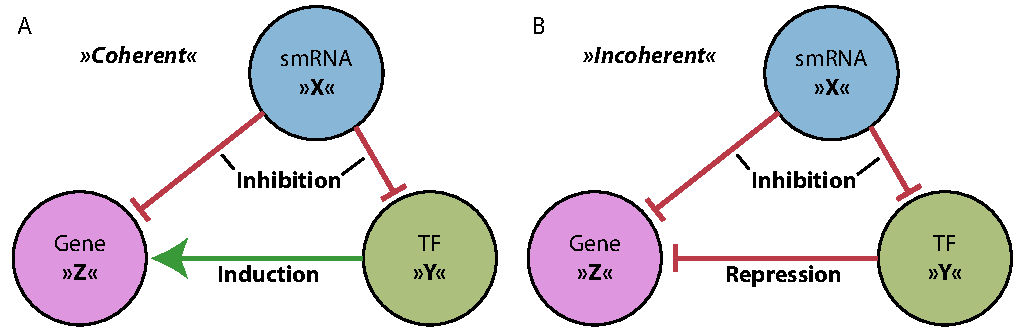
\includegraphics[width=\textwidth]{figures/ffl-theory}
\caption[Small RNA Feedforward Loop Theory.]{\textbf{Small RNA Feedforward Loop Theory.} The figure represents the two cases of smRNA FFLs most accessible to current analysis methods, i.e., the cases of smRNA (\textbf{X}) targeting of TF (\textbf{Y}) and ultimate gene (\textbf{Z}).  \textbf{A)} Basic coherent smRNA FFL. The smRNA (\textbf{X}) inhibits both the TF as well as the ultimate gene target. Since the TF (\textbf{Y}) is an activator of target gene (\textbf{Z}) expression, smRNA regulation has the same direct and indirect effect on ultimate gene expression. \textbf{B)} Basic incoherent smRNA FFL. The smRNA (\textbf{X}) has a direct suppressive effect on the target gene (\textbf{Z}), but the simultaneous suppression of the TF (\textbf{Y}), which in turn represses the target gene (\textbf{Z}), leads to elevation of target gene expression, ameliorating or even inverting the direct effect.
\label{fig:ffl-theory}}
\end{figure}

In the following, the principle of feedforward loops will be applied to transcriptomic and ontological analyses of gene expression in blood-borne cells after stroke. Pathways of co-regulated transcripts and their TFs will be identified by modularisation of a comprehensive FFL network in CD14$^+$ monocytes. The additional information leveraged from FFL-implied pathways will be ordered and interpreted based on previous studies on the identified pivotal actors.

\begin{method}

\subsection{Feedforward Loop Creation}
Starting from the set of differentially expressed TFs (p < 0.05) active in CD14$^+$ monocytes (as seen in Figure \ref{fig:smrna-tf-network-fractions}), single \acfp{ffl} of smRNAs (miRNA or tRF), TFs, and genes were detected using \emph{miRNeo} (as described in Query \ref{lst:loop}, Section \ref{sec:database:usage}). FFLs were created CD14$^+$ monocyte-specific by using only TF activity from these cells and by removal of any smRNAs not detected in CD14$^+$ cells in the Juzenas \emph{et al.}\cite{Juzenas2017} data set. Additionally, because of the high amount of TF$\to$gene relationships in CD14$^+$ cells, TF relationships were filtered for the 10\% with highest activity.

\subsection{Visualisation and Modularisation}
The network of all smRNAs, TFs, and genes included in these FFLs was visualised in gephi\cite{Jacomy2014} as a two-dimensional force-directed map, using the ForceAtlas2 algorithm. At initial network creation, tRFs were represented by the seeds included in their sequences, which were later associated with the mature tRFs. Using a community detection algorithm\cite{Blondel2008}, the network was sub-classified into five module classes (using edge weights and a resolution of 1.5, Modularity coefficient = 0.482).

\subsection{Module-specific Functions via GO Analysis}
 The module classification was reimported into R, and using R/topGO,\cite{Alexa2006} the functions of individual submodules were assessed by testing the significantly differentially expressed genes (adjusted p < 0.05) from each module against a background of 2000 randomly selected genes. Significant terms were manually screened, and differentially expressed genes were extracted from the test data for relevant terms.

\end{method}

\subsection{Feedforward Loop Network of CD14$^+$ Monocytes} \label{sec:stroke:ffl-cd14}
The complete FFL network of TFs DE in stroke patient blood (p < 0.05) was created using \emph{miRNeo} and visualised in gephi. In total, 195\,043 unique FFLs were discovered, 193\,803 containing miRNAs, and only 1240 containing tRFs. After filtering of the top 10\% of TF$\to$gene relationships by activity, 19\,309 miRNA- and 169 tRF-FFLs remained. These FFLs constitute a network of 2628 nodes and 22\,456 edges (Figure \ref{fig:cd14-ffl-modules}). Community detection\cite{Blondel2008} resulted in a sub-classification of nodes into five distinct modules, which were subsequently analysed for their functions using GO.

The reasoning behind this approach is to explain in more detail the findings of GO enrichment analysis of the differentially expressed large transcripts (compare Section \ref{sec:stroke:large-rna-go}), and to more closely define the pathways implicated in the context of smRNA regulatory modules. In applying feedforward loops, there may be an increase in identification of biologically relevant pathways, as opposed to network creation by TF$\to$gene and smRNA$\to$gene relationships alone. Notably, there was no cross-talk of modules across significant GO terms; if a term was found significant in GO enrichment analysis of a module, all genes associated with the term were located in the same module. The following paragraphs will attempt to interpret the terms associated with each module to shed some light on the distribution of their functions and possible inter-module cooperations.

Particular attention was paid to GO terms indicating a direction (e.g., »positive regulation«), which in combination with the direction of differential expression of the implicated genes may give an indication of the tangible effect of module gene regulation after stroke. When writing of »module genes«, differential expression (adjusted p-value < 0.05) of these genes in stroke patient blood is always implied.

\begin{figure}
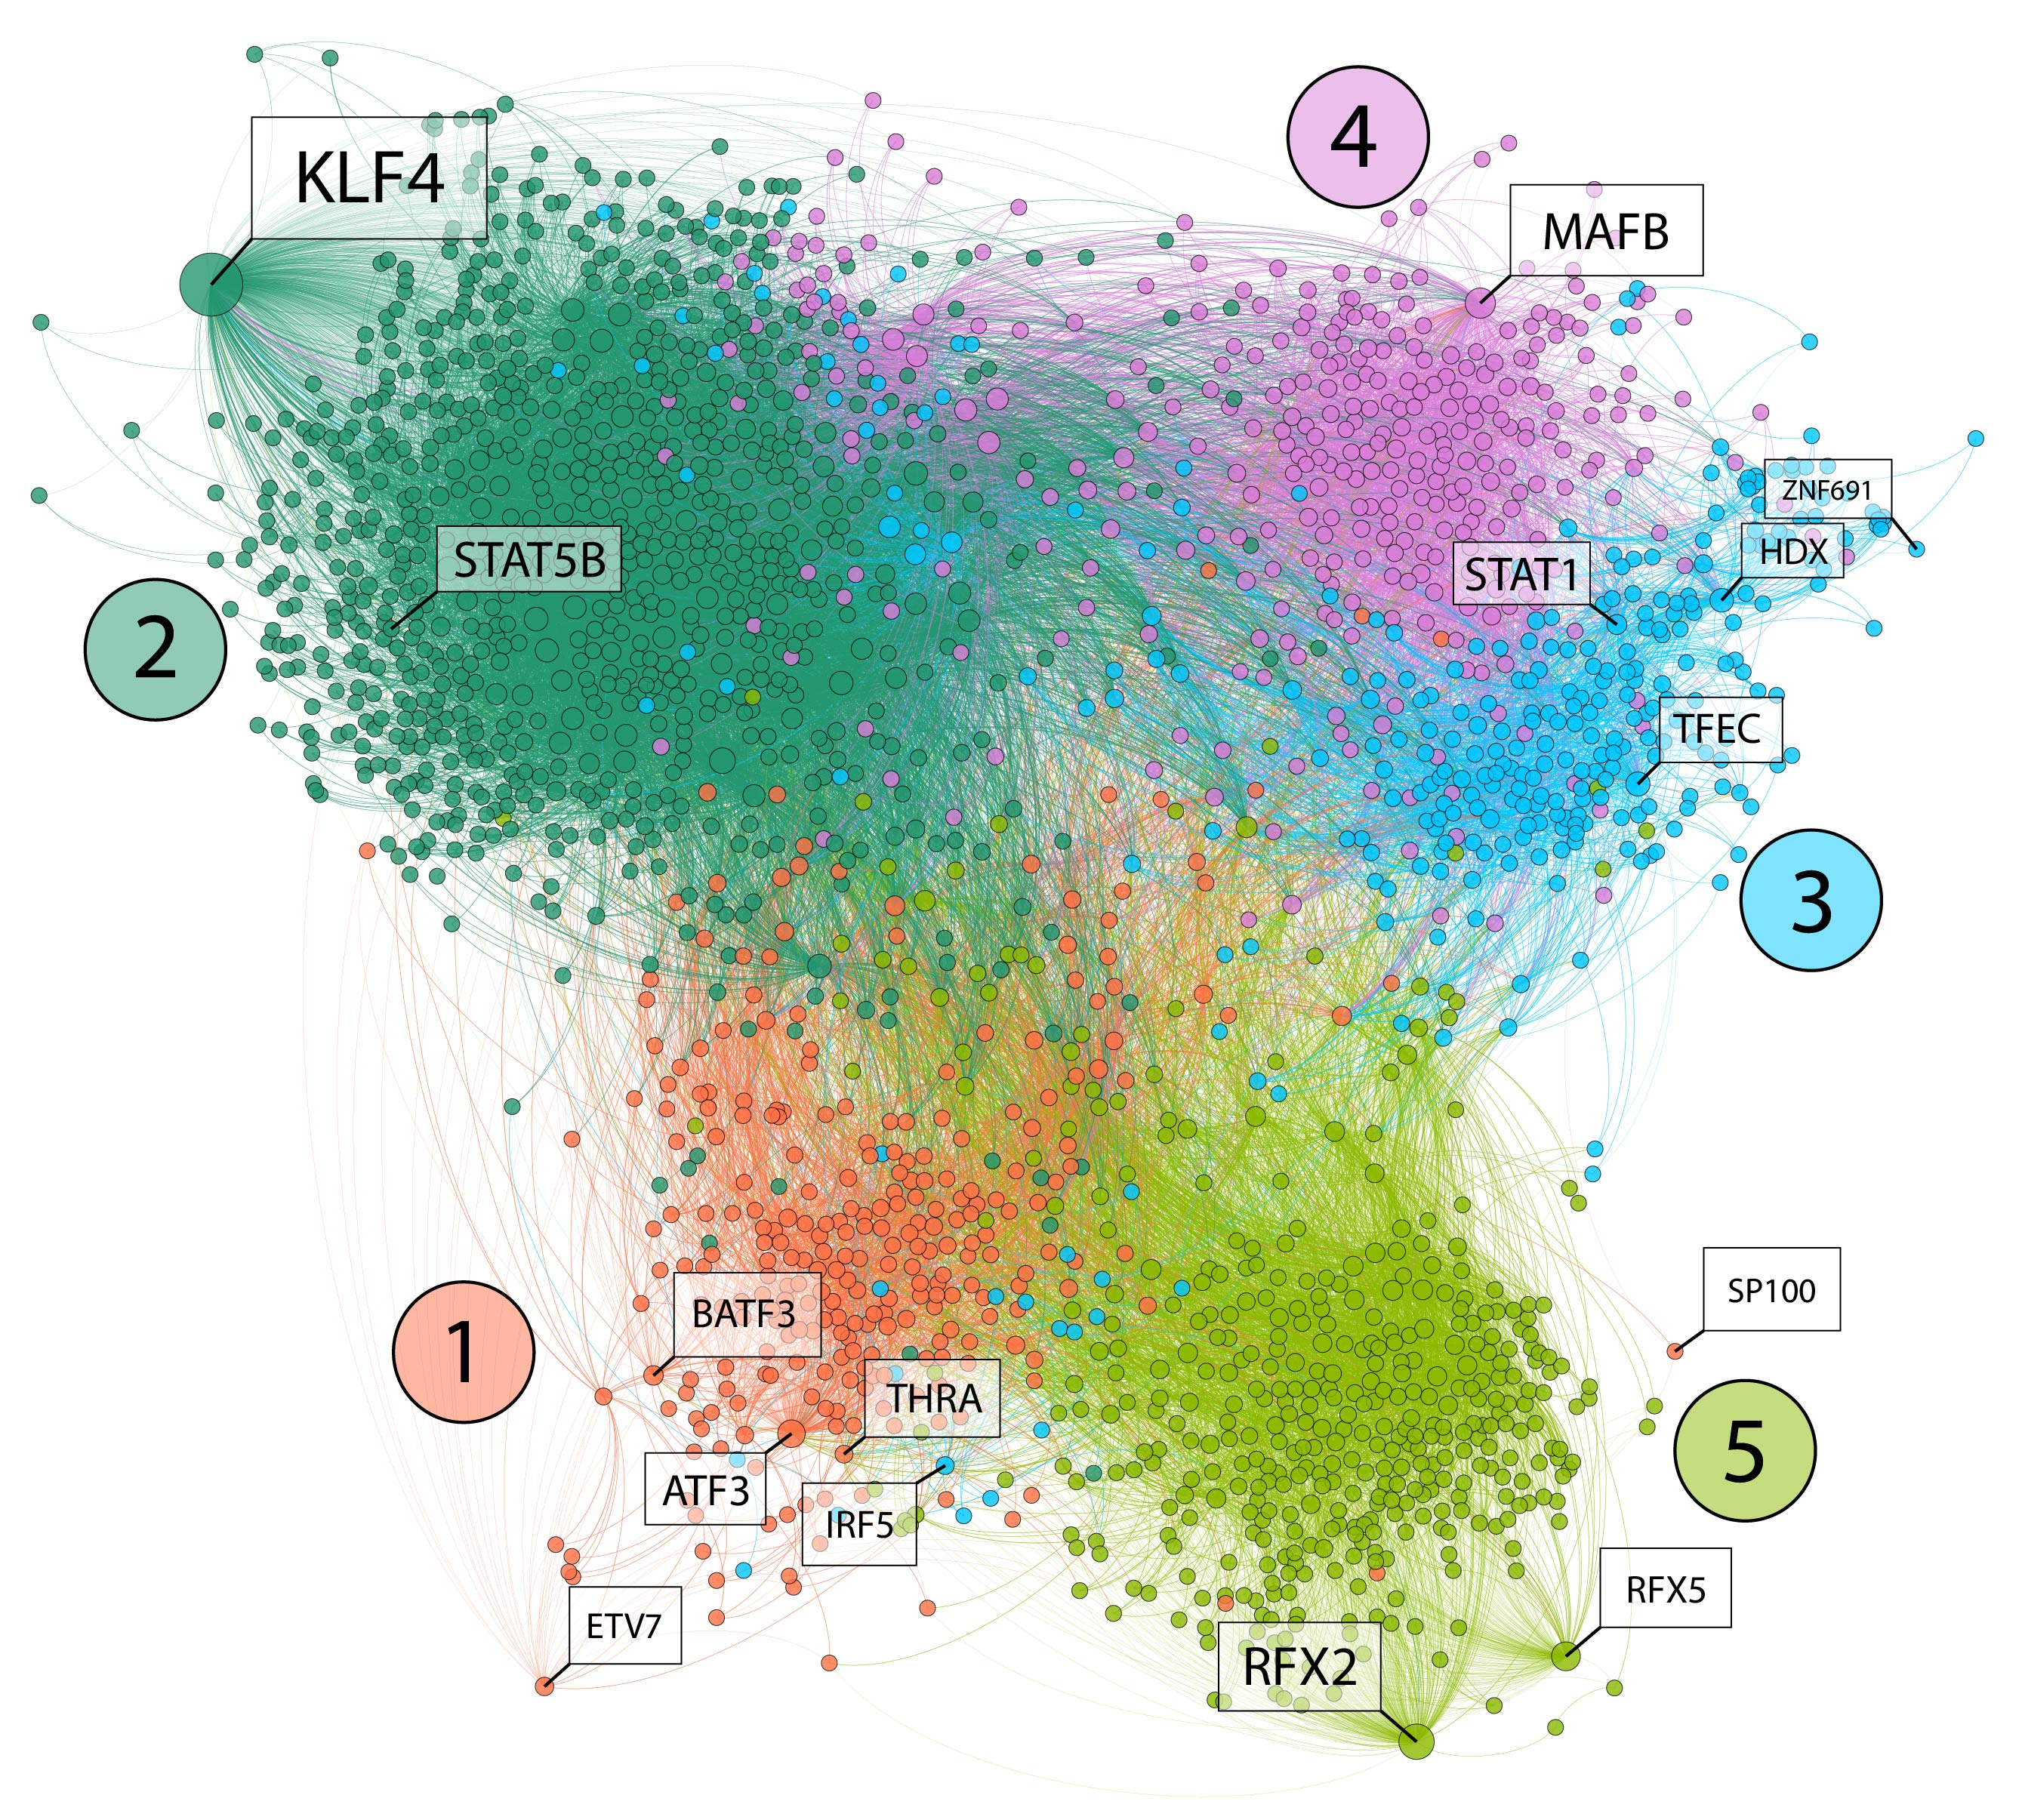
\includegraphics[width=\textwidth]{figures/cd14-ffl-modules}
\caption[Complete Feedforward Loop Network of Differentially Expressed Transcription Factors in CD14$^+$ Monocytes.]{\textbf{Complete Feedforward Loop Network of Differentially Expressed Transcription Factors in CD14$^+$ Monocytes.} Feedforward loops (FFLs) were created by \emph{miRNeo} query of transcriptional interaction of transcription factors (TFs), miRNAs, and tRFs towards all genes, but limited to FFLs of which the regulatory elements (TFs and smRNAs) were present and active in CD14$^+$ monocytes, and additionally filtered for the top 10\% TF$\to$gene relationships by activity. The resulting network was assembled in a force-directed 2D-projection and analysed to yield modularity information. The algorithm identified 5 distinct modules of small and large RNA FFLs, indicated by colours and numbers in circles. TFs differentially expressed in stroke patient blood are marked with a name tag (node size denotes differential expression count-change of TFs). 
\label{fig:cd14-ffl-modules}}
\end{figure}

\subsubsection{Module One}
GO enrichment analysis of significantly DE genes from module one resulted in 16 GO terms from 35 DE genes. The most significant biological process governed by module one is »negative regulation of transcription« with eight \acp{sg} and an adjusted p-value of \me{1.6}{4}. The second- and third-most significant terms indicate an influence on apoptotic processes (p = 0.0021 and 0.0049) with three \acp{sg}, which are a subset of genes from the first term, \emph{SP100}, \emph{SKIL}, and \emph{ATF3}. Further, module one genes are implicated in positive regulation of GTPase activity (5 SGs, p = 0.0069), epithelial cell differentiation (5 SGs, p = 0.0088), cellular response to IFN-$\upgamma$ (2 SGs, p = 0.024), platelet degranulation (2 SGs, p = 0.033), and cellular response to IL-1 (2 SGs, p = 0.049).

Apart from \emph{SP100} (major constituent of PML-SP100 bodies, see module three), \emph{SKIL} (part of SMAD pathway, regulating cell growth and differentiation), and \emph{ATF3} (member of the broadly acting CREB family of transcription factors), frequently implicated genes include \emph{CCL2} (chemokine ligand for CCR2, exhibits chemotactic activity for monocytes\cite{Zhang1994}) and \emph{CAMK1} (broadly acting calmodulin-dependent protein kinase, involved e.g. in the ERK cascade). All above \acp{sg} are down-regulated in stroke patient blood (own results).

\emph{SP100} is induced by IFNs, presents with potent antiviral and tumour suppressor effects, and has been shown to induce apoptosis via the extrinsic pathway together with \emph{FLASH} or caspase-2 and p53 in \emph{PML} nuclear bodies (see module three).\cite{Sanchez-Pulido2007} A reduction of \emph{SP100} expression would thus likely lead to inhibition of apoptotic events. Histone deacetylase (\emph{HDAC}) inhibition (compare module five) suppresses the IFN-mediated \emph{SP100} up-regulation.\cite{Vlasakova2007} Recently, \emph{SP100}, \emph{STAT1} (compare module three), and \emph{KLF4} (compare module two) were found to be co-elevated in the peripheral monocytes of tobacco-smoking (but not in non-smoking) HIV-positive patients and associated with an increased depressive index.\cite{Lorenz2019}

\emph{SKIL}, also known as SnoN, is known as a pro-apoptotic mediator that can bind and activate p53, and is targeted by mir-30 family members, which can ameliorate its apoptotic effect.\cite{Kim2018} Conversely, Smad3, a pro-apoptotic protein, is repressed in synergy by \emph{STAT3} and the \emph{SKIL} paralog c-Ski.\cite{Makino2017} A recent study has identified \emph{SKIL} at the heart of a feedforward loop including \emph{EGR1} and hsa-miR-124-3p in the blood of schizophrenia patients, which showed a down-regulation of \emph{EGR1} and \emph{SKIL}, and concomitant up-regulation of miR-124-3p.\cite{Xu2016} However, in post-stroke whole blood, \emph{EGR1} and miR-124-3p are unchanged (own results).

\emph{ATF3} also shows a pro-apoptotic effect, it can be activated by stress mediator p38 MAPK;\cite{Song2016} reduction of \emph{ATF3} in a cell model via siRNA interference reduced apoptosis.\cite{Sun2017} \emph{ATF3} is a key regulator of macrophage IFN responses, it represses pro-inflam"-ma"-to"-ry pathways (e.g. IL-6, TLR), and is also induced by IFNs. Correspondingly, \emph{ATF3}-deficient mice are more susceptible to endotoxin-mediated shock by cytokine overproduction. \emph{ATF3} and \emph{CXCL10} (compare module two) are co-induced by IFNs.\cite{Labzin2015} \emph{ATF3} sustains \emph{STAT3} phosphorylation through inhibition of phosphatases, and thus amplifies IL6-gp130-STAT3 signalling.\cite{Glal2018} \emph{ATF3} down-regulates \emph{ACHE} expression during stress by binding to the consensus recognition site of cyclic-AMP responsive element binding (CREB) proteins, »TGACGTCA«. In this case, a non-enzymatic, pro-apoptotic function of \emph{ACHE} is stipulated.\cite{Heinrich2018} Similarly, \emph{ATF3} attenuates hypoxia-induced apoptosis by down-regulating the expression of the pro-apoptotic factor carboxyl-terminal modulator protein (CTMP), via binding to the ATF/CREB site in the CTMP-promoter.\cite{Huang2015}

Module one genes, which decrease translational activity, are in the majority down-regulated, which may indicate a positive influence on transcriptional mechanisms, in line with the facilitation of a response to the insult. Given the uncertainty of whether the transcription factors of module one act as activators or repressors (FANTOM5 data only supplies binding probability, not mode of action), the real picture likely is more complicated, with mixed outcomes in expression regulation. A major component of module one processes is apoptotic signalling, which the top three (down-regulated) genes, \emph{SP100}, \emph{SKIL}, and \emph{ATF3}, are all involved in. All three genes are oncogenes, and as such involved in cell cycle control. While module one genes present a complex regulatory picture, the function of the three most-involved genes may be summarised as pro-apoptotic; their consistent down-regulation in patient blood after stroke thus implies an inhibition of apoptotic processes inside module one. Additionally, \emph{SP100} and \emph{ATF3} present with clear ties to cholinergic processes, in their involvement with neurokines and STATs, association with nicotine consumption, and the attenuation of \emph{ACHE} expression. 

\subsubsection{Module Two}
Module two, being the largest module, predictably also offers most process-related terms (50 GO terms, 34 SGs), of which most are related to immunity or basic processes of cell physiology. For the sake of clarity, immunity-related terms will be explored first. Module two genes most significantly participate in regulation of response to cytokine stimulus (4 SGs, p = \me{2.9}{4}), response to LPS (5 SGs, p = \me{5.6}{4}), inflammatory response (6 SGs, p = 0.0015), and T- and B-cell differentiation (2 SGs each, p = 0.036 and 0.041). The highest DE genes from module two involved in these processes are \emph{SORL1} (a known regulator of neurokine signalling), \emph{STAT5B}, the IL-10 receptor $\upalpha$, \emph{PLXNB2} (involved in cell migration),  \emph{JAK2}, the transcription factor \emph{KLF4} (with many broad functions, but implicated in MAPK/ERK cascades and IL-4 mediated macrophage differentiation\cite{Ghaleb2017}), \emph{PTPN2} (phosphatase involved in dephosphorylating JAKs and STATs), and \emph{CXCL10} (pro-inflammatory chemokine ligand implicated in response to brain injury by activating microglia).
 
Non-immune physiological terms refer to regulation of cell migration (8 SGs, p = \me{1.4}{4}), negative regulation of MAPK cascade (4 SGs, p = \me{4.7}{4}), cellular response to peptide (5 SGs, p = \me{9.5}{4}), nucleus organisation (3 SGs, p = 0.0010), erythrocyte differentiation (3 SGs, p = 0.0010), negative regulation of cell adhesion (4 SGs, p = 0.0015), regulation of ERK cascade (3 SGs, p = 0.0085), regulation of angiogenesis (3 SGs, p = 0.013), regulation of cold-induced thermogenesis (2 SGs, p = 0.031) and several more basic processes. Many of these processes appear to be vital to the immune functions described above, as they share many of the most highly DE genes, such as \emph{SORL1}, \emph{STAT5B}, \emph{PLXNB4}, \emph{KLF4}, and \emph{PTPN2}. 

Module two includes several genes directly involved in the JAK/STAT immune response, such as \emph{IL10RA}, \emph{JAK2}, \emph{STAT5B}, and \emph{PTPN2}; module two genes are mostly down-regulated except for \emph{SORL1} (which shows dramatic increase in terms of count-change) and \emph{STAT5B} (own results).

\emph{SORL1} gives rise to the protein SorLA, synonymous with LR11, a transmembrane receptor that can interact with a wide variety of ligands intra- as well as extra-cellularly.\cite{Yin2015} SorLA is primarily known as the neuronal ApoE4 receptor, and thus widely associated with AD risk. Among other functions, it regulates APP trafficking and processing, and is significantly decreased in the AD-vulnerable regions of late-onset AD patients.\cite{Yin2015} However, in addition to its well-studied neuronal roles, it is highly expressed on the surface of monocytes and macrophages, and additionally up-regulated in acute myeloid leukaemia.\cite{Sakai2012} SORL1 binds many immune-related ligands such as the neurokine IL-6 and soluble neurokine receptors IL6R and CNTFR, mediating their cellular uptake. It associates with the transmembrane IL-6 receptor and reduces downstream effects via a reduction in STAT3 phosphorylation.\cite{Larsen2017} Conversely, while decreasing \emph{cis} signalling as just described, SORL1 may increase \emph{trans} signalling, i.e., IL6 availability in the blood stream which then binds to the soluble IL6 receptor and can affect any cell possessing the ubiquitously distributed gp130.\cite{Rabe2008} It has been shown that overexpression of a soluble gp130 form can effectively suppress inflammation mediated by the soluble IL6 receptor without interfering with the function of the transmembrane IL6 receptor.\cite{Rabe2008}

\emph{PLXNB2} can promote inflammation via activation of the NF-$\upkappa$B pathway.\cite{Zhang2018} In addition, it prominently mediates a plethora of the functions of angiogenin (ANG): it is the receptor for ANG in physiological and pathological cells; ANG acts though \emph{PLXNB2} on cell proliferation; \emph{PLXNB2} modifies ANG RNA-processing activity and cell type specificity (see Section \ref{sec:intro:trfs}); and \emph{PLXNB2} mediates neuroprotective effects of ANG.\cite{Yu2017} Moreover, \emph{PLXNB2}-deficient macrophages showed greater mobility and would healing capabilities than WT cells.\cite{Roney2011} A recent study shows its close association to inflammation-related circulatory events: upon inflammatory stimulation (using TNF-$\upalpha$, IL-1$\upbeta$, IL-4, and IL-6) of murine and human cells, endothelium-derived extracellular vesicles carrying miRNAs were released and taken up by monocytes causing decreased monocytic \emph{PLXNB2} levels and increased splenic monocyte mobilisation.\cite{Akbar2017} Twelve miRNAs were enriched in these vesicles, most of which show high differential expression in stroke patient blood (own results in brackets); these are hsa-miRs: -632 (not detected in stroke), -126-3p (\ac{lfc} = -1.12, p = \me{3.0}{11}), 151a-3p (\ac{lfc} = -2.37, p = \me{5.6}{22}), -26b-5p (\ac{lfc} = -1.17, p = \me{5.0}{5}), -126-5p (\ac{lfc} = -2.23, p = \me{5.2}{7}), -7a-5p (\ac{lfc} = -0.54, p = 0.03), -1972 (not detected), -15b-5p (\ac{lfc} = -0.85, p = \me{5.2}{7}), -23a-3p (\ac{lfc} = -1.68, p = \me{9.9}{16}), -374b-5p (\ac{lfc} = -1.85, p = \me{1.3}{5}), -23b-3p (\ac{lfc} = -1.73, p = \me{1.2}{17}), and -7b-5p (\ac{lfc} = 0.73, p = \me{4.1}{6}).

\emph{KLF4} has gained much attention since it was discovered to be one of the four factors for induction of pluripotent stem cells (iPSCs, induced by OCT3/4, SOX2, MYC, and KLF4).\cite{Takahashi2006} In macrophages (often using the model RAW264.7), \emph{KLF4} controls activation in response to LPS stimulation by regulating, among others, NF-$\upkappa$B, TGF-$\upbeta$, IL-1$\upbeta$, and HMGB1, at least partly through Smad3 inhibition (compare module one).\cite{Feinberg2005,Liu2008,Liu2012} In monocytes, \emph{KLF4} regulates differentiation towards a pro-inflammatory type of resident monocytes, such that \emph{KLF4} KO mice completely lacked inflammatory monocytes in blood and spleen.\cite{Feinberg2007,Alder2008,Kurotaki2013}
%interacts with sumo (sp100, pml)

The protein tyrosine phosphatase \emph{PTPN2} is implied in IL-1$\upbeta$-mediated inflammation. Mice deficient of \emph{PTPN2} die few weeks after birth because of anaemia, colitis, and severe systemic inflammation. Macrophages depleted of \emph{PTPN2} show excessive inflammasome activation. \emph{PTPN2} reduction leads to more general inflammation, but also less tumour susceptibility, likely because of a more efficient eradication of oncogenic cells.\cite{Spalinger2018} Increased inflammatory cascades following \emph{PTPN2} reduction are likely caused by the decrease in \emph{STAT1} and \emph{STAT3} dephosphorylation, and the concomitant increase in STAT signalling (compare module five, \emph{HDAC7}).\cite{Kim2018a}
 
In summary, module two genes seem to be responsible for facilitating an adequate immune response by regulating basic processes in order to enable immune cells to fulfil their functions (e.g., response to cytokines and cellular mobility). \emph{SORL1} up-regulation suppresses STAT3 activation, but putatively increases IL-6 availability in the blood stream, thereby pushing a whole-body immune activation. \emph{PLXNB2} reproducibly is reduced in response to inflammatory signalling, which leads to higher-func"-tion"-ing monocytic cells. \emph{PTPN2} reduction likewise is associated with a higher-func"-tion"-ing immune system and increased inflammatory cascades via an inhibition of STAT inactivation. \emph{KLF4} reduction may indicate a pro-differentiation signal, generating mature immune cells to interfere with the infarction. In addition, \emph{PLXNB2} interferes with \ac{ang} function, and thus may directly impact tRF generation. 

\subsubsection{Module Three}
Module three, with 14 GO terms and 13 SGs, appears similar in principle to module two, although much fewer basic physiological terms are involved. This is explained by the smaller size of the test set; the ontologies for basic terms include substantially more genes, and the likelihood of significant enrichment in the test set is reciprocal to test set size. The most significant biological processes of module two genes involve cellular response to IFN-$\upgamma$ (3 SGs, p = \me{1.6}{4}) and positive regulation of transcription (5 SGs, p = \me{9.1}{4}), as opposed to negative regulation of transcription found in module one. Further, module three genes are involved in the cytokine-mediated signalling pathway (4 SGs, p = 0.0018), regulation of IFN production (2 SGs, p = 0.0034), JAK-STAT cascade (2 SGs, p = 0.0048), negative regulation of angiogenesis (2 SGs, p = 0.0056), regulation of innate immune response (2 SGs, p = 0.035), and positive regulation of cytokine production (2 SGs, p = 0.048). Most frequently occurring genes are \emph{STAT1}, \emph{PLSCR1} (implicated in amplification of IFN response), \emph{PML} (also associated with IFN- and TNF-responses), and \emph{IRF5} (implicated in TLR7/8-induced induction of IFNs and other pro-inflammatory cytokines). All \acp{sg} of module three are down-regulated in stroke patient blood (own results).

Phospholipid scramblase 1 (\emph{PLSCR1}) is an oncogene implicated in cell cycle control, apoptosis, and mediation of antiviral response. While its mechanism of action is yet unexplained, the mature protein localises to the nucleus and has been shown to bind DNA.\cite{Ben-Efraim2004} While it does not induce apoptosis on its own, its overexpression has inhibitory effects on several cell cycle controllers and anti-apoptotic proteins such as Bcl-2.\cite{Huang2006} \emph{PLSCR1} participates in the antiviral response by potentiating IFN activity, which increases expression of a subset of \acp{isg}, including STAT1.\cite{Dong2004} It is expressed in human macrophages and monocytes, in which it is increased in systemic inflammatory conditions, and seems to also contribute to pro-thrombotic conditions.\cite{Suzuki2010,Herate2016} 

Promyelocytic leukaemia protein (\emph{PML}) is, together with \emph{SP100} (see module one), the major constituent of PML nuclear bodies, that are also known as \ac{nd10}. These small nuclear organelles are known for their peculiar and enigmatic function in antiviral response, which they seem to convey by a wide variety of molecular functions, from chromatin modification to physical trapping of virus particles.\cite{} Recently, however, they have also been connected to a direct regulation of innate immune responses. IFN therapy increases the expression of both \emph{PML} and \emph{SP100}, and enhances their antiviral activity.\cite{Regad2001} Correspondingly, \emph{PML} depletion reduces the capacity of IFNs to interfere with viral infection.\cite{Chee2003} PML has the capacity to modulate different stages of the pathway from IFNs through ISGs to the activation of STATs by associating with and stabilising transcription factor complexes, for instance by binding directly to \emph{STAT1} and \acp{irf} (see below).\cite{Chen2015} The production of IL-1$\upbeta$ and IL-6 is significantly reduced in \emph{PML}-deficient cells;\cite{Lo2013} and correspondingly, \emph{PML}-deficient mice are resistant to LPS-mediated lethality.\cite{Lunardi2011} This directly links to an epigenetic switch that leads to cellular transformation: inflammation, through NF-$\upkappa$B, activates Lin28 and rapidly reduces let-7 miRNA levels. This leads to de-repression of the IL-6 mRNA, and the increased IL-6 peptide conveys cellular transformation through \emph{STAT3} activation, as well as positive feedback by inducing NF-$\upkappa$B synthesis.\cite{Iliopoulos2009}

\emph{IRF5}, a well-studied member of the Interferon Regulatory Factor transcription factor family, is an important element of most blood-borne immune cell types, particularly of macrophages and pro-inflammatory monocytes.\cite{Li2016} It has been demonstrated that \emph{IRF5} is involved in transcriptional induction of IL-6, IL-12, and TNF-$\upalpha$ mediated by the \acf{tlr}/\ac{myd88} complex. \emph{IRF5}-deficient mice also show resistance to LPS-mediated lethality (compare PML/SP100).\cite{Takaoka2005} While KO-mice showed severely impaired production of the aforementioned cytokines, IFN-$\upalpha$ production was not impaired; the responsible interferon-stimulated response elements have yet to be determined.\cite{Takaoka2005} \emph{IRF5} is highly expressed in monocytes and macrophages as well as B cells and dendritic cells, and its expression is induced by a pro-inflam"-ma"-to"-ry environment.\cite{Krausgruber2011} On the spectrum of macrophage states after differentiation, \emph{IRF5} (together with \emph{IRF1} and \emph{IRF8}) is involved in the commitment to a pro-inflammatory (M1) phenotype (as opposed to the »wound healing« M2 type).\cite{Chistiakov2018}  The M1 phenotype is brought about by increased activity of NF-$\upkappa$B and STAT1, whereas the M2 counterpart is induced by IL-4-, IL-10-, and IL-13-mediated STAT3 and STAT6 signalling.\cite{Wang2014a} Molecular competition for MyD88 binding between IRF5 and IRF4 is crucial for the determination of pro- (\emph{IRF5}) or anti-inflammatory (\emph{IRF4}) differentiation.\cite{Negishi2006} Thus, a down-regulation of IRF5 together with unchanged levels of IRF4, as is the case in stroke patient blood (own results), would lead to anti-inflammatory conditions in monocyte and macrophage populations. M1$\to$M2 macrophage transition supports resolution of inflammation and tissue healing; reduction of IRF5 expression in monocytes and macrophages via siRNA interference improved healing after myocardial infarctions and skin wounds in mice, in parallel with a reduction of the pro-inflammatory cytokines IL-1$\upbeta$, IL-6, and TNF-$\upalpha$.\cite{Courties2014}

Module three genes (implicated in positive regulation of transcription, but all down-regulated) appear to act in partial opposition to module one genes (implicated in negative regulation of transcription, and all down-regulated), thus possibly being part of homeostatic events surrounding gene transcription in response to inflammatory events. Modules one and three also share GO terms involved in responses to, and production of, interferons and interleukins.

In summary, module three seems to be representative of immune suppression via several mechanisms; mediation of pro-inflammatory signalling via INFs is repressed, and IRF5 suppression may induce an anti-inflammatory, pro-resolving differentiation of monocytes and macrophages; cytokines and STAT signalling are likewise down-regulated; ND10 nuclear bodies are repressed. On the other hand, pro-apoptotic signalling may be de-repressed via PLSCR1 reduction.

\subsubsection{Module Four}
Module four, with 12 significant GO terms from 7 SGs, is a fairly small module, which is nevertheless highly associated with immune processes; most significantly, genes of module four convey positive regulation of innate immune response (2 SGs, p = 0.0039) and positive regulation of cytokine production (2 SGs, p = 0.0075); more accurately, IL-1 production (1 SG, p = 0.038). Further, module four genes show association with negative regulation of myeloid cell differentiation (1 SG, p = 0.038), positive regulation of response to cytokine (1 SG, p = 0.038), myeloid cell homeostasis (1 SG, p = 0.042), positive regulation of inflammatory response (1 SG, p = 0.045), and negative regulation of myeloid leukocyte differentiation (1 SG, p = 0.049). The most prevalent SGs in these terms are \emph{GBP5} (activator of the NLRP3 inflammasome assembly), \emph{MAFB} (transcription factor required for monocyte differentiation), and \emph{ZBP1} (cytoplasmic DNA-sensor which activates downstream IFN production in activated macrophages). All above \acp{sg} are down-regulated in stroke patient blood (own results).

\emph{GBP5} (for Guanine Nucleotide Binding Protein) is a molecular marker for the classically activated, pro-inflammatory M1 type macrophage,\cite{Fujiwara2016} and a critical factor for the assembly of the \emph{NLRP3} inflammasome.\cite{Shenoy2012} \emph{GBP5} is strongly induced by IFNs through NF-$\upkappa$B, and in turn induces expression of IFNs and pro-inflammatory cytokines such as IL-6 and TNF-$\upalpha$.\cite{Feng2017} Consequently, it plays a critical role in response to viral infection, e.g. by Influenza or HIV, as well as diverse other pathogens.\cite{Feng2017,Krapp2016} In mice, miR-21-5p inhibition led to an increase in macrophage GBP5, with a concomitant increase in TNF-$\upalpha$ and a decrease in the anti-inflammatory IL-10.\cite{Corsetti2018} However, in stroke patient blood, both miR-21-5p and GBP are down-regulated (own results).

\emph{MAFB} is a transcription factor with critical roles in macrophage differentiation and function, and specific for mononuclear phagocytes in all cells of the haematopoietic system.\cite{Hamada2020} Macrophages deficient in \emph{MAFB} and \emph{MAF} reacquire the ability for self-renewal, but only upon concomitant up-regulation of two pluripotent stem cell-inducing factors, \emph{KLF4} and \emph{MYC} (compare module two).\cite{Aziz2009} However, in stroke patient blood (own results), \emph{KLF4} is reduced while \emph{MAF} and \emph{MYC} are unchanged. After induction of ischemic stroke, macrophage-specific \emph{MAFB}-deficient mice showed excessive sterile inflammation, likely due to a failure in clearing of \acp{damp}.\cite{Shichita2017} The authors found \emph{MAFB} to be a critical controller of the macrophage scavenger receptor 1 (MSR1), which in turn is essential for the clearance of DAMPs after ischemic stroke, and is also down-regulated in stroke patient blood (own results, \ac{lfc} = -3.54, p = \me{2.9}{6}). Additionally, retinoic acid receptor agonist \emph{Am80} increased \emph{MAFB} and \emph{MSR1} expression in the delayed phase of ischemic stroke, and had ameliorating effects on stroke pathology.\cite{Shichita2017} \emph{miRNeo} query of retinoic acid receptor interactions in CD14$^+$ cells indicates \emph{RARA}, the $\upalpha$ retinoic receptor, as most active towards MAFB (lower activity also exhibited by \emph{RARG} and \emph{RXRA}). \emph{RARA} also targets STATs 1, 5A, and 5B, as well as \emph{ACHE} and \emph{IL6ST} (also known as gp130) in these cells. 

An \emph{ex vivo} experiment of \emph{MAFB} inhibition by siRNA in human CD14$^+$ monocytes found an elevation in IRF3 phosphorylation and concomitant increase in INF-$\upalpha$ and INF-$\upbeta$ production.\cite{Liu2019} \emph{MAFB} also seems responsible for direct regulation of all genes of the C1q complement complex, which activates the classical component pathway.\cite{Tran2017} Thereby, and by regulation of the Axl protein, \emph{MAFB} is essential for efferocytosis, the phagocytosis of apoptotic cells \emph{in vivo}.\cite{Sato2018} \emph{MAFB} is regulated by diverse pathways; immunological mediators (e.g. cytokines), lipid metabolism, and miRNAs.\cite{Hamada2020} Two miRNAs experimentally identified as regulating \emph{MAFB}, miR-152\cite{Tozaki-Saitoh2019} and miR-155\cite{Jablonski2016}, are significantly down-regulated in stroke patient blood (own results; hsa-miR-152-3p: \ac{lfc} = -1.97, p = \me{2.0}{11}; hsa-miR-155-5p: \ac{lfc} = -0.69, p = \me{6.5}{4}). miR-155 has additionally been shown to induce pro-inflammatory macrophages, while \emph{MAFB} itself promotes anti-inflammatory M2-type macrophage differentiation.\cite{Kim2017} In CD14$^+$ monocytes, MAFB interacts with \emph{CHRNA6}, \emph{IL6}, the \emph{IL6} receptor, and \emph{STAT1} (via \emph{miRNeo}, from Marbach \emph{et al.}\cite{Marbach2016} regulatory circuits). In summary, \emph{MAFB} reduction after stroke may contribute to a shift towards pro-inflam"-ma"-to"-ry M1\-/type macro"-phages, prolonged activity of which may inhibit efferocytosis and the M2-mediated healing process in the delayed phase.

Z-DNA binding protein 1 (\emph{ZBP1}, also known as \emph{DAI}) is an IFN-induced cytoplasmic sensor of \acp{damp} that positively mediates various forms of programmed cell death, general pro-inflammatory events (such as cytokine production), and \emph{NLRP3} inflammasome assembly; however, its triggering ligands or molecular patterns are still unclear.\cite{Kuriakose2018} More recently, it was shown that \emph{ZBP1} is necessary for type-I and type-II IFN-mediated necroptosis (a programmed form of necrosis),\cite{Yang2019} by sensing viral as well as endogenous RNA (in addition to DNA), possibly in the unusual Z-conformation.\cite{Maelfait2017} 

Murine macrophages lacking the \ac{myd88} TLR adapter protein were able to undergo apoptosis via redundant TLR pathways mediated by \emph{ZBP1}. In contrast, KO of the type-I INF receptor, as well as of its downstream effectors \emph{STAT1} and \emph{IRF9}, abolished the macrophages' ability to undergo TLR-mediated \ac{myd88}-independent apoptosis.\cite{Kuriakose2016} Moreover, de-novo transcription and protein synthesis (compare »regulation of transcription« in modules one and three), as well as JAK1/STAT1 transcriptional activation are required for IFN-induced necroptosis through \emph{ZBP1} signalling.\cite{Yang2019} \emph{ZBP1}-deficient mice (via CRISPR/Cas-9 KO) were significantly protected from acute IFN-mediated \acf{sirs},\cite{Yang2019} making the \emph{ZBP1} down-regulation in stroke patient blood (own results, \ac{lfc} = -1.70, p = 0.001) a logical bodily response to prevent \acf{cids}, and a possible component of the counter-regulation, \acf{cars} (see Section \ref{sec:intro:stroke}). Notably, NF-$\upkappa$B signalling blocks type-II IFN-induced necroptosis (compare modules two and three).\cite{Thapa2011}

%homointeraction and RIPK3 interaction of ZBP1?

In summary, module four constitutes a small, largely anti-inflammatory module, conveying an attenuation of inflammatory processes by limiting the sensing of inflammatory stimuli (\emph{ZBP1}), activation of inflammatory pathways, inflammasome assembly and cytokine production (\emph{GBP5}), and clearance of DAMPs in the infarct area (\emph{MAFB}). However, GO terms also indicate a positive influence on differentiation of monocytes. For instance, the decrease in \emph{MAFB} expression may promote a delayed phenotypic shift towards M1-type macrophages, which may have a deleterious effect on patient recovery.

\subsubsection{Module Five}
Module five is a medium-sized module (29 GO terms from 18 SGs) and highly involved with stroke-relevant processes, most importantly, vascular permeability. Most terms relate to basic molecular functions of the cell, such as regulation of cell-substrate adhesion (3 SGs, p = 0.0037), cellular component maintenance (2 SGs, p = 0.0052), membrane depolarisation (2 SGs, p = 0.0052), regulation of protein tyrosine kinase activation (2 SGs, p = 0.0063), positive regulation of small molecule metabolism (2 SGs, p = 0.0063), fatty acid metabolic process (3 SGs, p = 0.0064), positive regulation of lipid metabolic process (2 SGs, p = 0.010), regulation of cytokine production (3 SGs, p = 0.022), response to hypoxia (2 SGs, p = 0.027), and several more. The genes most highly implicated in these processes are \emph{SRC}, \emph{ABCD1}, and \emph{HDAC7}. Module five SG expression is mixed in stroke patient blood; of the most prevalent genes, \emph{SRC} and \emph{ABCD1} are down-regulated, and \emph{HDAC7} is up-regulated.

Src, from the \emph{SRC} gene, is a well-studied kinase from the larger family of Src kinases implicated in diverse physiological processes. Increased \acf{vp}, i.e., a loss of blood-brain-barrier function, can be induced by TNF-$\upalpha$, IL-1$\upbeta$, IL-6, and \ac{vegf}. Of relevance, Src controls \ac{vegf} expression after ischemic stroke, thereby modulating \ac{vp}. Reduction of Src (but not Src family kinase Fyn) activity in mice via complete congenital KO or pharmacologic inhibition (using the synthetic inhibitor PP1) resulted in a reduction of permanent \ac{mcao}-induced stroke volume of 50\% and up to 70\%, respectively. This beneficial effect was associated with a prevention of \ac{vp}.\cite{Paul2001} In these experiments, Src inhibition seemed to restore perfusion and oxygenation in the penumbra (the region adjacent to the infarct), protecting the surrounding tissue. Later, these VEGF-modulating effects of Src on \ac{vp} and stroke recovery were replicated in rats with transient infarction.\cite{Zan2014} In another set of experiments, it was shown that the neuroprotective effect of ischemic postconditioning in mice probably depends on Src kinase activation.\cite{Kumar2014b} In a human cellular model, Src was up-regulated upon inflammatory TNF-$\upalpha$ signalling and conveyed increases in \ac{vp} in a p38 MAPK-dependent manner (compare module one, \emph{ATF3}).\cite{Adam2016} Src family kinases can physically bind to gp130, phosphorylate STAT3,\cite{Brown1996} and are intricately involved with TLR-CD14 signalling, in an »important but not obligatory« manner.\cite{Okutani2006} 

\emph{ABCD1} is a member of the \ac{abc} superfamily of active transporters, responsible for the transport of very long chain fatty acids, and implicated in inflammatory processes by its influence on peroxisomal $\upbeta$-oxidation.\cite{Hama2018} It is best known for its role in \ac{ald}, where an \emph{ABCD1} deficiency leads to microvascular perfusion anomalies in the brain.\cite{Lauer2017} The working hypothesis states that \emph{ABCD1}-related up-regulation of adhesion molecules in the endothelium causes higher leukocyte interaction and thus impairs blood flow in the capillaries. Notably, carriers of the ApoE4 allele are more significantly affected by \ac{ald} (compare module two, \emph{SORL1}).\cite{Orchard2019} Most molecular changes caused by the deficiency are likely a result of impaired fatty acid transport into peroxisomes. \emph{Abcd1}-deficient mice show a dramatically altered brain region-specific phospholipid profile.\cite{Hama2018}

\emph{HDAC7} (histone deacetylase 7) is a protein responsible for deacetylating histones and non-histone proteins, with regulatory implications in cell proliferation, apoptosis, differentiation, and migration.\cite{Lei2017} \emph{Hdac7}$^{-/-}$ mice are embryonic lethal because of an angiogenetic failure leading to rupture of blood vessels.\cite{Chang2006} It has been shown that the HDAC7 protein directly interacts with STAT3, deacetylation of which interferes with its ability to dimerise, thus impairing its functionality.\cite{Peixoto2016,Lei2017} \emph{HDAC7} was also found to induce an apoptotic gene program and c-Myc suppression upon ectopic expression in human SD-1 cells.\cite{Barneda-Zahonero2015} \emph{HDAC7} additionally suppresses macrophage genes relevant for phagocytosis, TLRs, interleukins and TNF pathway genes by acting as a transcriptional repressor of myocyte enhancer factor \emph{MEF2C}.\cite{Barneda-Zahonero2013} In human C10 cells reprogrammed to macrophages, \emph{HDAC7} expression significantly inhibited the expression of TNF-$\upalpha$, IL-1$\upbeta$, and IL-6.\cite{Barneda-Zahonero2013} VEGF stimulates HDAC7 phosphorylation, leading to its aggregation in the cytosol and subsequent suppression of angiogenesis mediated by matrix metalloproteases (MMT) 10 and 14, which degrade proteins essential for vessel integrity.\cite{Miano2006,Ha2008} \emph{HDAC7} can also directly associate with \emph{RARA} (see module four, \emph{MAFB}) to form a repressor complex that inhibits, among others, miR-10a.\cite{Lee2017} This inhibition led to de-repression of pro-inflammatory signalling via \emph{GATA6} and \emph{VCAM1}, with negative impact on \ac{vp} in vascular endothelia.
 
In summary, module five genes seem to be primarily associated with vascular permeability and the integrity of the blood-brain-barrier. Reduction of \emph{SRC} may be beneficial in regard to stroke volume, whereas the effects of \emph{ABCD1} decrease on vessel integrity are less clear. Secondarily, down-regulation of \emph{SRC} and \emph{ABCD1} may have a negative impact on lipid metabolism, with consequences for lipid-mediated signalling. \emph{HDAC7} up-regulation, on the other hand, may constitute a pro-apoptotic signal.

\subsection{Transcript Clustering by smRNA:TF:gene Feedforward Loops \\Increases Informative Resolution of Gene Set Enrichment Analyses} \label{sec:stroke:resolution}
In principle, the analysis of separate modules represents changes brought on by DE TFs in stroke patient blood, focused on CD14$^+$ cells by analysing feedforward loops comprising smRNAs and TF-in"-ter"-ac"-tions specific to CD14$^+$ cells. An advantage of the separation via FFL association is a reduction in dimensionality, which may make the implications of each module more accessible than a complete list of all changed genes or TFs in the experiment, and may also increase the informative resolution of the GO enrichment analyses. Visual inspection of Figure \ref{fig:cd14-ffl-modules} indicates a partition between modules two and four on the top, and modules one and five on the bottom of the map. The role of module three is visually less clear. Module three is the module most »intermingling« with the other modules, particularly in the case of \emph{IRF5}, which spatially is closer to module one and five than it is to three (see Figure \ref{fig:cd14-ffl-modules}, bottom). More generally, there are two zones of module three intermingling, between modules one and five, and between modules two and four.

Visual representation of the GO terms derived from non-modularised analysis versus the terms collected from module analyses clearly shows the proposed advantage regarding informative resolution of the method (Figure \ref{fig:gsoap-ffl}). The non-modularised version shows less terms, that are also less specific (Figure \ref{fig:gsoap-ffl}\,A, reproduced from Figure \ref{fig:gsoap-de}), while the module-derived terms are higher in number, and also refer to more specific processes (Figure \ref{fig:gsoap-ffl}\,B). Intriguingly, this t-SNE visualisation of GO terms shows a central cluster around module one, comprising terms from all other modules. Since the similarity of terms is calculated via their shared genes, this may indicate that processes involving cooperation of modules are grouped in the center, while module-specific processes cluster at the edges. Correspondingly, module three terms cluster on the left side in close vicinity of this central cluster, while module two and module five terms are located in opposite areas on the graph.

\begin{figure}
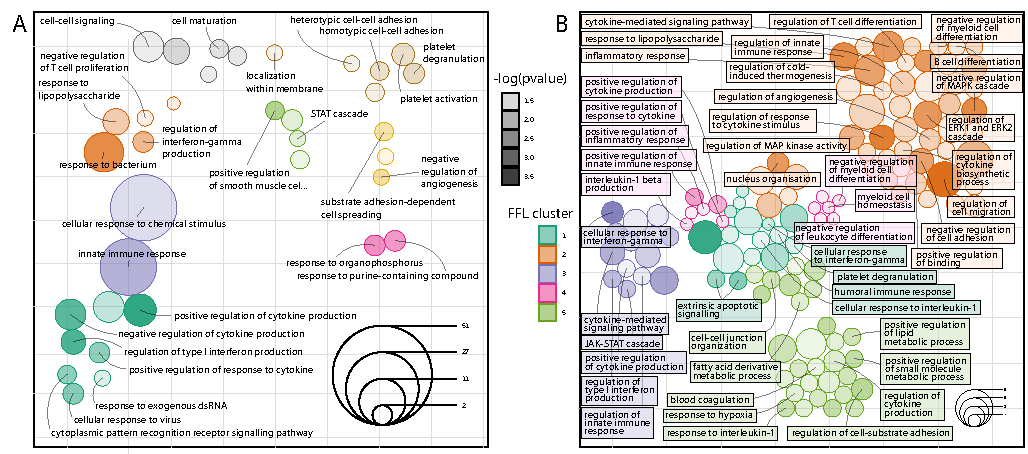
\includegraphics[width=\textwidth]{figures/gsoap-ffl}
\caption[FFL module Gene Ontology Enrichment.]{\textbf{FFL module Gene Ontology Enrichment Increases Informative Resolution.} A comparison between GO enrichment performed on (A) differentially expressed (DE) genes and (B) DE genes classified by FFL network modules shows similar biological processes but increased information depth. Size denotes number of significant genes in term, colour indicates p-value (all p < 0.05). \textbf{A)} DE genes with absolute ac{lfc} > 1.4 are enriched in processes of immunity and circulation. Cluster colour derived from t-SNE similarity. Reproduction of Figure \ref{fig:gsoap-de}. \textbf{B)} t-SNE mapping of GO terms derived from analysis of single FFL modules shows details of involvement with immune processes and basic cellular function. Colour indicates original FFL module (see text). The middle cluster, comprised of parts from all modules surrounding module 1, may signify an »area of cooperation« between the modules.
\label{fig:gsoap-ffl}}
\end{figure}

The most prevalent themes of module function are inflammatory events, in particular those mediated by TLR/MyD88-associated pathways, IFN responses, and interleukin and TNF-$\upalpha$ signalling. Many of these innate immune pathways are important in sterile inflammation as well as in response to viral infection. This is in concert with the fact that the most prevalent genes identified by module GO analysis are pivotal regulators of immunity. Other themes implied by the analysis are apoptotic/necroptotic events, transcriptional activation, lipid metabolism and signalling, and blood vessel integrity. In most cases, the participating forces are representative of activation as well as inhibition, again underscoring the homeostatic aspect of these regulatory processes.

Inflammation as a common theme is represented in all modules, with diverging implications. Modules one, two, and five may be described as pro-inflammatory modules, while anti-inflammatory properties dominate in modules three and four. The module topology of the two-dimensional force-directed map of FFLs (see Figure \ref{fig:cd14-ffl-modules}) replicates this pro- versus anti-inflammatory dichotomy, indicating that the innate immune response may be the defining factor in FFL modularisation (Figure \ref{fig:cd14-ffl-annot}). Module one conveys pro-inflammatory signals via the de-repression of IFN response through \emph{ATF3}, module two via the increase in IL6 availability through \emph{SORL1}, the decrease in STAT dephosphorylation by \emph{PTPN2}, and the decrease in \emph{PLXNB2}, which may be mediated by smRNA-carrying vesicles and is associated with splenic monocyte mobilisation. In module five, \emph{HDAC7} in association with \emph{RARA} may repress miR-10a, which in turn de-represses pro-inflammatory mediators. Modules three and four, on the other hand, may be described as largely anti-inflammatory. Module three presents inhibition of IFN signalling via the suppression of \emph{PLSCR1} and \emph{STAT1}, \emph{PML/SP100} nuclear bodies, and \emph{IRF5}. Down-regulation of module four genes may convey attenuation of inflammation through \emph{GBP5}, \emph{MAFB} (and the related \emph{MSR1}), and \emph{ZBP1} suppression. Attenuation of inflammation after stroke may be a bodily response to prevent \acf{sirs}, however, exaggerated response or external intervention harbours the danger of \acf{cars} and \acf{cids}.

\begin{figure}
\includegraphics[width=\textwidth]{figures/cd14-ffl-annot}
\caption[Complete Feedforward Loop Network of Differentially Expressed Transcription Factors in CD14$^+$ Monocytes, Annotated.]{\textbf{Complete Feedforward Loop Network of Differentially Expressed Transcription Factors in CD14$^+$ Monocytes, Annotated.}  A reproduction of Figure \ref{fig:cd14-ffl-modules} annotated with most pertinent molecular functions as identified via individual module GO analysis. Distance to the center of the graph of each annotation resembles the distribution of the category across all modules (closer to the center - more common functional class), and functions shared by two modules are indicated by their annotation across the intersecting lines. The most common functional classes refer to inflammation, apoptosis, and STAT regulation.
\label{fig:cd14-ffl-annot}}
\end{figure}

Influences on apoptotic/necroptotic events are also distributed between several modules. Module one conveys anti-apoptotic signals via reduction of \emph{SP100}, in agreement with \emph{PML} reduction in module three. Additionally, \emph{PLSCR1} down-regulation in module three may have an indirect anti-apoptotic effect through de-repression of anti-apoptotic proteins such as Bcl-2. \emph{ZBP1} in module four is a \ac{damp} sensor that can induce necroptosis independently of MyD88, however, it is suppressed in stroke patient blood and requires STAT1 signalling (which is also suppressed), and de-novo protein synthesis. Transcriptional activation is regulated by genes in modules one and three, but the final effect of their competition cannot be assessed with certainty. \emph{HDAC7} up-regulation in module five, on the other hand, may induce a pro-apoptotic program.

Lipid metabolism and blood vessel integrity are implied specifically in module five. Peroxisomal $\upbeta$-oxidation of very long chain fatty acids is reduced through the inhibition of \emph{ABCD1}, with consequences in lipid mediator signalling (e.g., regulation of \emph{MAFB}) and inflammation. However, the bottom line effect of module five gene reactions to stroke in regard to blood vessel stability, i.e., the question if \emph{SRC}, \emph{ABCD1}, and \emph{HDAC7} regulation are beneficial or detrimental to vascular integrity, is still largely unclear and a worthwhile subject for further studies.

Another common theme of module gene processes is the involvement and regulation of signal transducers and activators of transcription, \acp{stat}. Many SGs are inducers of STATs (\emph{PLSCR1}, \emph{IRF5}, \emph{RARA}, \emph{MAFB}), binding partners (\emph{SKIL}, \emph{PML}), or involved in activation or deactivation via phosphorylation/dephosphorylation and acetylation/deacetylation (\emph{ATF3}, \emph{SORL1}, \emph{PTPN2}, \emph{SRC}, \emph{HDAC7}). Thus, homeostasis of STAT transcription and activation seems to play an important role in the observed processes. Of note, STAT1 is decreased in stroke patient blood, but STAT3 is not differentially regulated. However, effects mediated by modulators of activity, such as sustained STAT3 phosphorylation via \emph{ATF3} (module one), reduced STAT3 phosphorylation via \emph{SORL1} (module two), increased STAT3 phosphorylation via \emph{PTPN2} (module two) and \emph{SRC} (module five), or STAT3 deacetylation via \emph{HDAC7} (module five) can have dramatic impacts on cellular function without a change in STAT3 expression. Additionally, the studies cited on STAT control via phosphorylation and acetylation are not comprehensive, so some of the implied proteins may interact with STATs other than STAT3. In stroke patient blood, changes are seen in STAT1 (down-regulated), STAT2 (down-regulated), and STAT5B (up-regulated).

Among module functions is also the control of blood cell differentiation, particularly of monocytes and macrophages. Both cell types can be driven towards a pro- or an anti-inflammatory phenotype via expression and activation of certain mediators. \emph{KLF4} (module two) drives monocytes towards a pro-inflammatory phenotype, and \emph{IRF5} (module three) mediates commitment to the pro-inflammatory M1-phenotype of macrophages in response to IFN signalling. Their concomitant down-regulation may thus produce an anti-inflammatory, pro-resolving phenotype of monocytic immune cells. Additionally, \emph{IRF5}-mediated M1-commitment is conveyed by STAT1 signalling, which is impaired through \emph{STAT1} down-regulation, whereas M2-commitment is mediated by STAT3 and STAT6 signalling, both of which are unimpaired. On the other hand, \emph{MAFB} (module four) expression drives commitment to the anti-inflammatory M2 type, and thus, its down-regulation may convey an opposite signal to \emph{KLF4} and \emph{IRF5} regulation. 

A number of module SGs also show cholinergic association: apart from the cholinergic/neurokine interface connecting IL6, gp130, and JAK/STAT to cholinergic properties of immune cells and neurons,\cite{Lobentanzer2019a} \emph{ATF3} down-regulates \emph{ACHE} which interferes with its stipulated non-enzymatic, pro-apop"-to"-tic function; \emph{RARA} induces \emph{STAT1}, gp130, and \emph{ACHE}, and \emph{MAFB} induces \emph{CHRNA6}, \emph{IL6}, \emph{IL6R}, and \emph{STAT1}. Other module cross-associations include module one/module three cooperation in regard to PML/SP100 nuclear bodies, \emph{SP100} and \emph{STAT1} co-elevation in monocytes of tobacco-smoking HIV-positive patients, and their antagonism in regard to the activation or deactivation of transcription. Module two and module four both have an impact on cell identity and differentiation via pluripotency-associated \emph{KLF4} and \emph{MAFB} signalling. Module one and module five are associated via the induction of SGs by p38 MAPK (\emph{ATF3} and \emph{SRC}), the ApoE4-association of \emph{SORL1} and \emph{ABCD1}, the support of \emph{HDAC7} in IFN-mediated \emph{SP100} up-regulation, and their opposite effect on apoptotic signalling. All of these associations (1-3, 1-5, 2-4) can be retraced in the FFL module visualisation (Figure \ref{fig:cd14-ffl-annot}).

%module one: %anti-apoptotic, transcriptional activation (required for ZBP1 necroptosis), %pro-inflammatory
%sp100 nd10 nbs tie to m3
%skil cooperates with stat3
%atf3 down-regulates ACHE, %sustains stat3 phosphorylation

%module two: increase in inflammatory signalling and response to inflammation, 
%pro-differentiation
%sorl1 reduces STAT3 phosphorylation via IL6R, increases IL6 availability, 
%apoe4 receptor
%ptpn2 dephosphorylates stats, down-regulation increases inflammation
%inflammation via smRNA vesicles decreased PLXNB2 and increased splenic monocyte mobilisation
%klf4 reduction is pro-resolve

%module three: %associated with IFN signalling, viral response; general suppression of inflammatory pathways IFN, TLR/MyD88, 
%commitment to M1 suppressed -> resolve
%plscr1 potentiates IFN signalling, induces STAT1; suppressed; 
%pro-apoptotic signalling de-repressed
%pml/sp100 nd10 bodies are induced by IFNs; suppressed
%pml binds STATs and IRFs, 
%ties to LPS
%IRF5 mediates IFN signalling, commitment to M1 phenotype (STAT1), as opposed to M2 (STAT3/STAT6), 
%MyD88 competition (IRF5->M1, IRF4->M2).;suppressed
%STAT1 itself is suppressed

%module four: %attenuation of inflammation, protection from SIRS
%GBP5 M1-macro marker; suppressed; inflammasome suppressed
%MAFB deficiency excessive sterile inflammation due to inefficient clearance of DAMPs; MSR1 also down; 
%RARA ties to STAT1, ACHE, gp130; MAFB ties to CHRNA6, IL6, IL6R, STAT1 (m3); 
%regulated by lipid metabolism (m5); 
%promotes M2 type; suppressed
%ZBP1 sensor of DAMPs, induced by IFN, necroptosis independent of MyD88, dependent on STAT1 and de-novo transcription (m1\&3), down-regulation protects from SIRS

%module five: %common theme blood vessel integrity, 
%stat homeostasis, %lipid metabolism brake, pro-apoptotic
%src gp130 stat phosphorylation, pharmacologic inhibition decreased stroke severity
%hdac7 deacetylates stat3, 
%associates with RARA
%abcd1 lipid carrier, association with apoe4

%module interactions
%m1/m3 antagonism/homeostasis?
%transcriptional activation
%sp100/pml nd10 bodies
%m2/m4 mafb/klf4 cell identity
%m1/m5 
%p38 induction of ATF3 and SRC
%apoe4 sorl1 and abcd1
%pro- vs anti-apoptotic

%small network of above genes?



%
%\section{Dimensionality Reduction and Correlation of Expression with Clinical Parameters}
%
%\begin{method}
%
%\subsection{WGCNA}
%Reduction of dimensionality of high-dimensional data, such as the expression of thousands of small RNA species and their correlation with clinical parameters of patients, can also be achieved by means of Weighted Gene Correlation Network Analysis (WGCNA, also R/WGCNA).\cite{Langfelder2008} The aim of this method is the identification of modules that group similarly-expressed genes. Each of these modules is represented by an eigenvector (called \emph{eigengene}), effectively replacing the individual expression parameters of the genes in the module. The eigengene can then be used to determine correlation of covariates to each module.
%
%To represent expression data in a network-based manner, the expression matrix is transformed into an adjacency matrix representing similarities between nodes, i.e., genes. The co-expression similarity $s_{ij}$ between two nodes $i$ and $j$ is defined as the absolute correlation coefficient between the expression profiles $$s_{ij} = |cor(x_i, x_j)|$$ with $x$ representing the node expression profile. A signed co-expression measure can be used to keep track of the direction of co-expression. Weighted networks allow the adjacency measures to assume continuous values between 0 and 1, thereby retaining the continuous nature of the underlying expression matrix. This is achieved by implementation of a soft threshold, which is usually chosen by the user to result in a scale-free network topology. The connectivity distribution in a scale-free network follows a power law, i.e., the probability of a node with $k$ connections is, for large values of $k$: $$P(k) = k^{-\alpha}$$ With $\alpha$ usually between 2 and 3. Many biological networks are assumed to be scale-free; however, this assumption has very recently been empirically questioned.\cite{Broido2019}
%
%Once the network is created, modules are identified via unsupervised clustering of densely connected nodes. Biological significance can then be assigned to each of the modules and genes. Module eigengenes can be calculated (the first principal component of the module) and correlated to traits, such as clinical parameters. In this manner, modules with potential functional implications can be identified.
%
%\subsection{Co-correlation}
%The fact that a subset of small \ac{seq} samples were also subjected to large \ac{seq} enables the application of a secondary correlation between those two approaches. For instance, module eigengenes derived from \ac{smrna} analysis can be correlated with the mRNA module eigengenes across the common patients. The module similarity $\sigma$ thus is defined as the correlation coefficient between eigengene profiles $e$ of modules $i$ and $j$: $$\sigma = |cor(e_i, e_j)|$$
%
%Significantly correlating modules (p < 0.05) were identified and further analysed downstream.
%
%%\section{Direct Interaction}
%
%\end{method}
%
%

